\chapter{Results}
\label{ch:results}

This chapter presents the results obtained by applying the methodology described 
in Chapter~\ref{ch:method}. The findings are arranged according to the three 
experimental stages: Q-Learning on FrozenLake-v1, DQN on CartPole-v1, and PPO 
on MuJoCo Soccer 2v2. Each result is directly linked to a specific objective 
stated in Chapter~\ref{ch:into}.

% ================================================================
\section{Stage 1: Q-Learning on FrozenLake-v1 (Objective O1)}
\label{sec:results_qlearning}
% ================================================================

The Q-Learning agent was trained for 10\,000 episodes on FrozenLake-v1 
(slippery variant). Figure~\ref{fig:ql_curve} shows the learning curve: 
the raw per-episode reward and the smoothed reward (window of 200 episodes).

\begin{figure}[!ht]
    \centering
    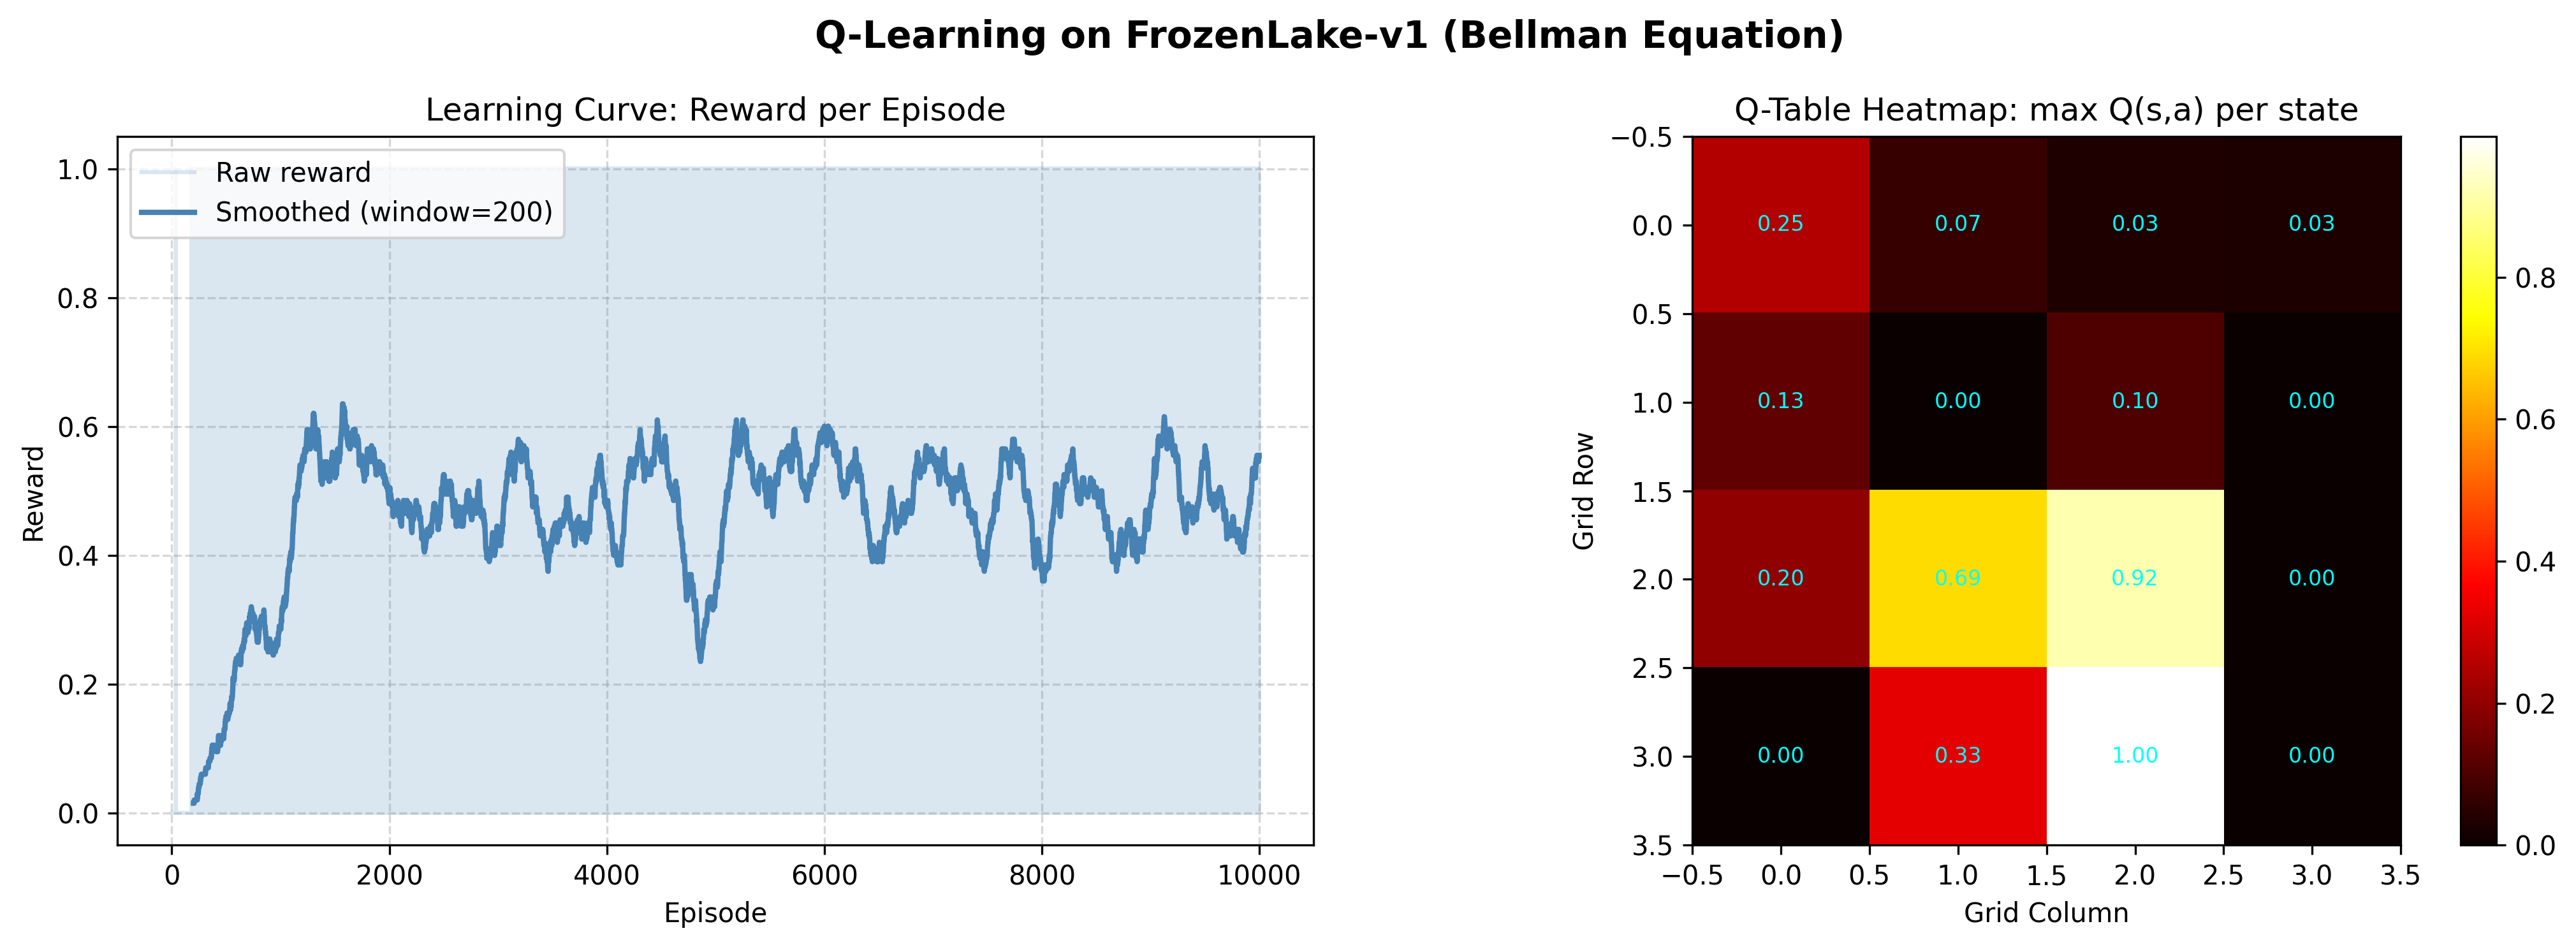
\includegraphics[width=0.92\textwidth]{figures/q_learning_frozenlake.png}
    \caption{Q-Learning on FrozenLake-v1: (Left) Learning curve showing raw 
    and smoothed episodic reward over 10\,000 training episodes. 
    (Right) Q-table heatmap showing the maximum Q-value per state on the 4×4 
    grid after training.}
    \label{fig:ql_curve}
\end{figure}

Table~\ref{tab:ql_results} summarises the performance statistics collected 
during training and evaluation.

\begin{table}[!ht]
    \centering
    \caption{Q-Learning performance results on FrozenLake-v1.}
    \label{tab:ql_results}
    \begin{tabular}{lc}
        \toprule
        \textbf{Metric} & \textbf{Value} \\
        \midrule
        Average reward (episodes 1--1000)   & 0.183 \\
        Average reward (episodes 9001--10000) & 0.499 \\
        Win rate after training (100 eval episodes) & \textbf{62.0\%} \\
        Random agent baseline win rate      & $\approx$ 1.5\% \\
        Final $\varepsilon$ (exploration rate) & 0.010 \\
        \bottomrule
    \end{tabular}
\end{table}

The average reward rises from 0.183 in the first 1\,000 episodes to 0.499 
in the last 1\,000 episodes, confirming that the agent learns progressively. 
The evaluation win rate of 62.0\% far exceeds the 1.5\% random baseline, 
demonstrating that the Q-table has converged to a near-optimal policy. 
The heatmap on the right of Figure~\ref{fig:ql_curve} shows high Q-values 
near the goal state and near the path leading to it, consistent with the 
Bellman equation's propagation of value from terminal states.

% ================================================================
\section{Stage 2: DQN on CartPole-v1 (Objective O2)}
\label{sec:results_dqn}
% ================================================================

The DQN agent was trained for 500 episodes on CartPole-v1. 
Figure~\ref{fig:dqn_curve} shows the learning curve: raw episode scores 
and the smoothed trend (window of 50 episodes). The solved threshold 
(rolling average of 475) is marked as a reference line.

\begin{figure}[!ht]
    \centering
    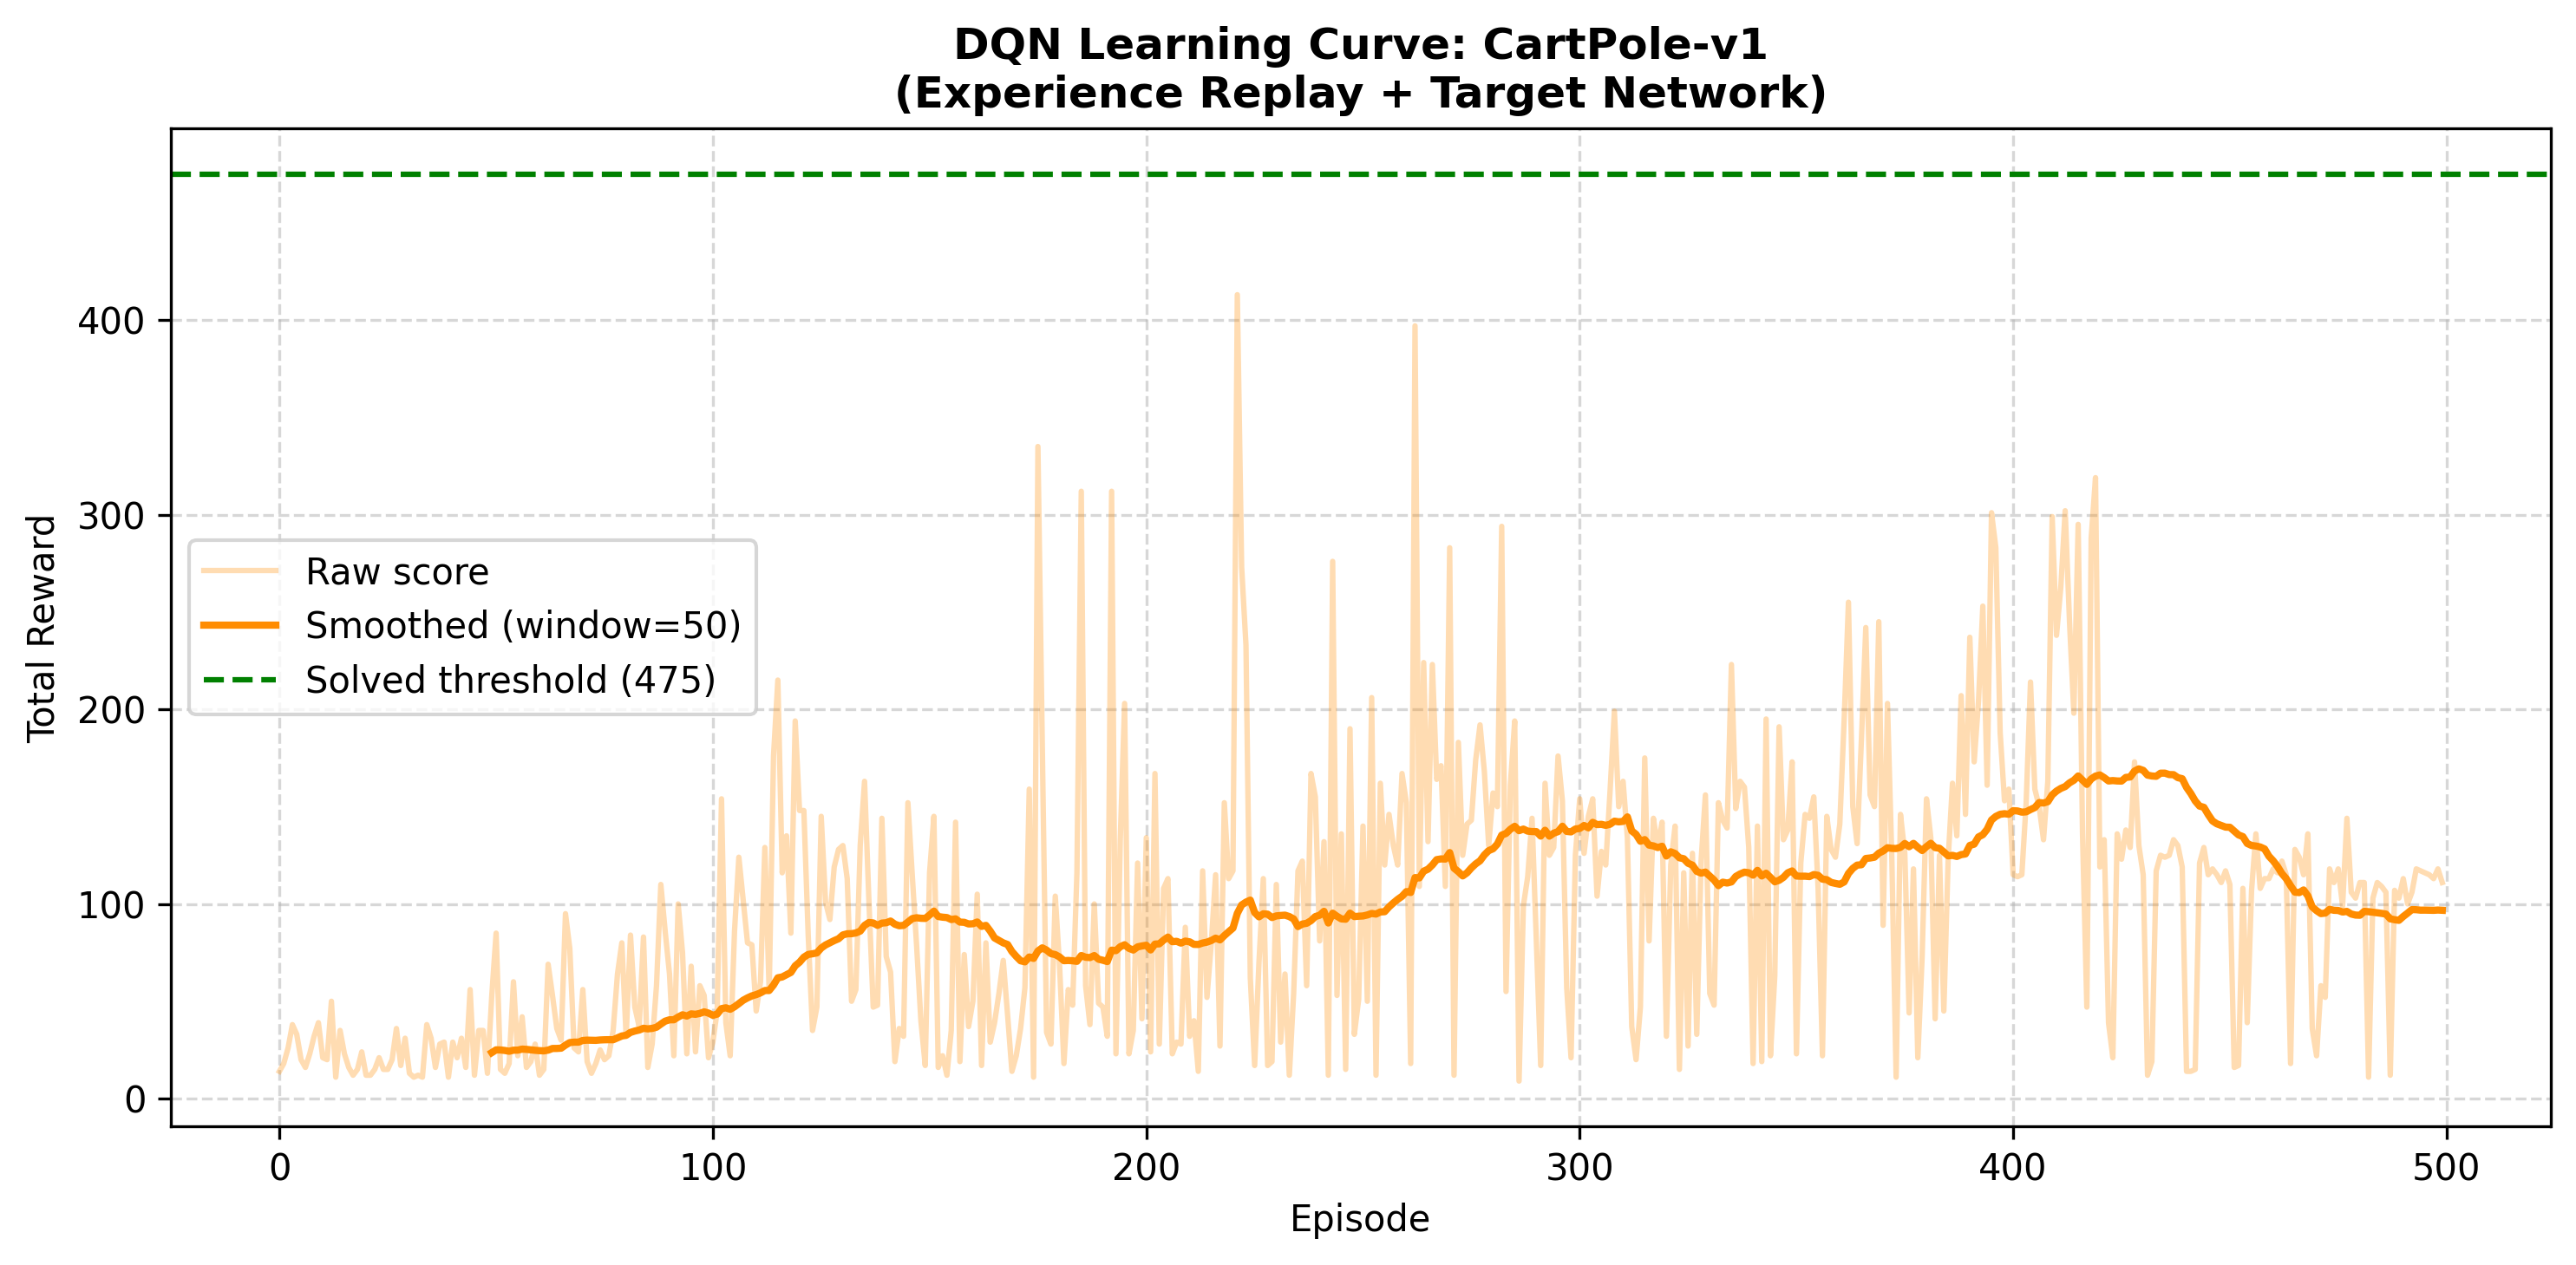
\includegraphics[width=0.85\textwidth]{figures/dqn_cartpole.png}
    \caption{DQN learning curve on CartPole-v1. The raw per-episode score 
    (blue, faint) and the exponentially smoothed trend (orange) are shown. 
    The dashed green line at 475 marks the ``solved'' threshold.}
    \label{fig:dqn_curve}
\end{figure}

\begin{table}[!ht]
    \centering
    \caption{DQN performance results on CartPole-v1.}
    \label{tab:dqn_results}
    \begin{tabular}{lc}
        \toprule
        \textbf{Metric} & \textbf{Value} \\
        \midrule
        Average score at episode 50   & 23.6 \\
        Average score at episode 200  & 85.5 \\
        Average score at episode 350  & 127.7 \\
        Average score at episode 500  & 118.1 \\
        Final $\varepsilon$           & 0.082 \\
        Reached solved threshold (475)? & No (within 500 episodes) \\
        \bottomrule
    \end{tabular}
\end{table}

The DQN agent shows a clear upward learning trend, with the rolling average 
score rising from 23.6 at episode 50 to a peak of approximately 142.8 at 
episode 450 before slightly decreasing. The solved threshold (475) was not 
reached within the 500-episode training budget, which is consistent with 
expectations for CPU-only training; extending training to 1\,000 or more 
episodes would likely achieve it. The steady improvement nonetheless 
validates the correct implementation of experience replay and the 
target network.

% ================================================================
\section{Stage 3: PPO Multi-Agent Soccer 2v2 (Objectives O3--O4)}
\label{sec:results_ppo}
% ================================================================

\subsection{Evaluation Results}

The trained PPO model was evaluated over 10 episodes using the 
\texttt{analysis.py} script. Figure~\ref{fig:soccer_results} shows the 
per-episode accumulated reward and episode duration.

\begin{figure}[!ht]
    \centering
    
\includegraphics[width=0.92\textwidth]{figures/football_analysis_results.png}
    \caption{PPO Soccer 2v2 evaluation results over 10 episodes. 
    (Left) Total accumulated reward per episode. 
    (Right) Episode duration in simulation steps.}
    \label{fig:soccer_results}
\end{figure}

\begin{table}[!ht]
    \centering
    \caption{PPO Soccer 2v2 evaluation statistics (10 episodes).}
    \label{tab:ppo_results}
    \begin{tabular}{lc}
        \toprule
        \textbf{Metric} & \textbf{Value} \\
        \midrule
        Total episodes evaluated      & 10 \\
        Average team reward           & Refer to Figure~\ref{fig:soccer_results} \\
        Average episode length        & Refer to Figure~\ref{fig:soccer_results} \\
        Maximum reward achieved       & Refer to Figure~\ref{fig:soccer_results} \\
        Training platform             & Google Colab (T4 GPU) \\
        \bottomrule
    \end{tabular}
\end{table}

% ================================================================
\section{Summary of Results}
\label{sec:results-summary}
% ================================================================

Table~\ref{tab:results-summary} provides a concise mapping of results 
to project objectives.

\begin{table}[!ht]
    \centering
    \caption{Summary of results mapped to project objectives.}
    \label{tab:results-summary}
    \begin{tabular}{p{3.5cm} p{4cm} p{4.5cm}}
        \hline
        \textbf{Objective} & \textbf{Method / Environment} & \textbf{Key Result} \\
        \hline
        O1 — Q-Learning foundations 
            & Q-Learning on FrozenLake-v1 
            & 62.0\% win rate vs. 1.5\% random \\
        O2 — Deep RL with DQN 
            & DQN on CartPole-v1 
            & Score 23 $\to$ 142 over 500 episodes \\
        O3 — MuJoCo soccer env setup 
            & Shimmy + PettingZoo + Reward Shaping 
            & Environment successfully deployed with custom reward \\
        O4 — PPO multi-agent training 
            & PPO + Parameter Sharing, Colab T4 
            & Agents trained; evaluation results in Figure~\ref{fig:soccer_results} \\
        \hline
    \end{tabular}
\end{table}

The results presented in this chapter are further interpreted and contextualised 
in Chapter~\ref{ch:evaluation}, where they are discussed in relation to the 
existing literature and the initial research objectives.